\section{Generalisation}\label{sec:generalisation}
In this section, we report experiments on CIFAR-10 and MNIST  datasets . Our aim here is to study the role of activations in generalisation performance of DNNs. In particular, we compare the generalisation performance of DNNs with adaptable gates (i.e., $A_t(\cdot,\cdot)$ changes with time) and DNNs with frozen gates (i.e., $A_t(\cdot,\cdot)=A_0(\cdot,\cdot),\forall t\geq 0$).%In the second part of this section, we present preliminary theory related to feature learning in DNNs.
%Another interesting observation is that, both zeroth-order and first-order activation terms are important. In particular, NPF indeed stores enough information, i.e., even if the gates are frozen and not adaptable, if they are copied a previously trained network, then we are able to recover good generalisation performance, however, not as good as adaptable gates.
Network Architecture and Hyper-parameters:
\textbf{Frozen Non-Learned gates generalise poorly:} We trained both ReLU and frozen-GaLU (in $\N_G(\Theta_t,\G(\N_R(\Tg_t)))$ we have $\Tg_t=\Tg_0,\forall t\geq 0$) networks on standard MNIST dataset to close to $100\%$ accuracy. We observed that the frozen-GaLU network trains a bit faster than the ReLU network. However, the test performances were around $96\%$ and  $98\%$ for frozen-GaLU and ReLU networks respectively\footnote{In the case of GaLU, in order to eliminate the effect of initialisation, we trained with identical as well as independent initialisation for the gating as well as the main network in the GaLU. }. We trained ReLU and GaLU networks on standard CIFAR-10 dataset close to $100\%$ training accuracy. In this case, the test performances were around $64\%$ and $72\%$ for GaLU and ReLU networks respectively.\hfill\\
\begin{comment}
Note that, in the case of $\N(\Tg_{\dagger},\infty;\Tv_t)$, we were initialising $\Tg_0\in \R^{d_{net}}$ and $\Tv_0\in \R^{d_{net}}$ in a statistically independent manner. Thus, in order to eliminate the effect of the initialisation, we also compared DGNs of the form  $\N(\Theta_t,\infty;\Theta_t)$ and $\N(\Tv_{\dagger},\infty;\Tv_t)$ (which we call as frozen ReLU networks). We trained both ReLU and frozen ReLU networks on standard MNIST dataset close to $100\%$ accuracy. The test performances were around $96\%$ and  $98\%$ for frozen ReLU and ReLU networks respectively. We trained ReLU and GaLU networks on standard CIFAR-10 dataset close to $100\%$ training accuracy. In this case, the test performances were around $72\%$ and $64\%$ for ReLU and frozen ReLU networks respectively.\hfill\\
\end{comment}
\textbf{Frozen Learned gates generalise better:} Note that, in these experiments, the frozen-GaLU network gates are copied from a gating network which is pre-trained, however, the weights $\Theta_0$ are initialised and trained again.  In the case of MNIST, 
In the case of CIFAR-10, frozen-GaLU with learned gates achieved a test performance of $70\%$, which is better than frozen-GaLU with non-learned gates with a performance of  $64\%$, and is however less than ReLU with performance of $72\%$. 

\begin{figure*}
\resizebox{\textwidth}{!}{
\begin{tabular}{ccc}
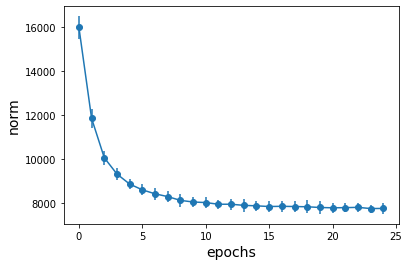
\includegraphics[scale=0.18]{figs/path-gram.png}
&
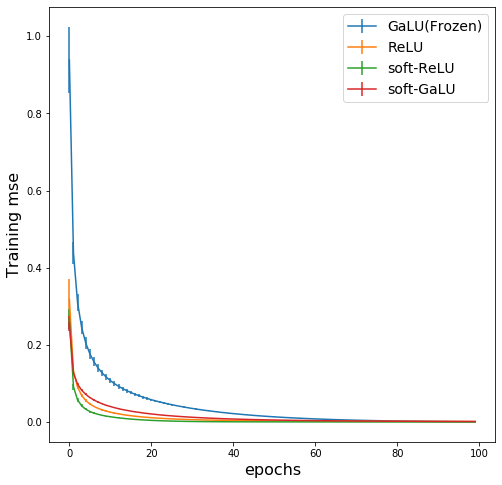
\includegraphics[scale=0.1]{figs/allnet-train.png}
&
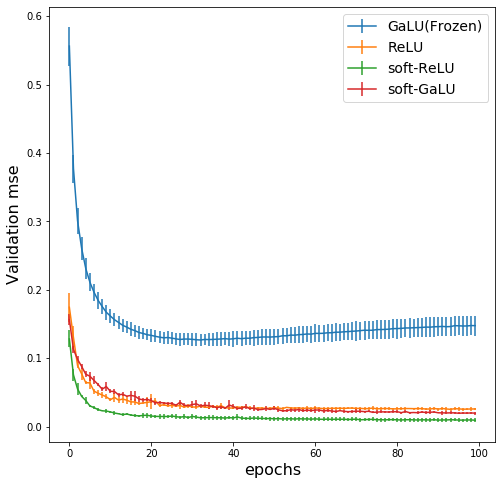
\includegraphics[scale=0.1]{figs/allnet-gen.png}
\end{tabular}
}
\caption{First two plots from the left show optimisation and generalisation in ReLU and GaLU networks for standard MNIST. The right most plot shows $\nu_t=y^\top (\widehat{H}_t)^{-1}y$, where $H_t=\Phi_t^\top \Phi_t$.}
\label{fig:gen}
\end{figure*}

\textbf{NPK dynamics in ReLU:} We consider ``Binary''-MNIST data set with two classes namely digits $4$ and $7$, with the labels taking values in $\{-1,+1\}$ and squared loss. We trained a standard DNN with ReLU activation ($w=100$, $d=5$). Recall that $H_t=\Phi^\top_t\Phi_t$  (the Gram matrix of the features) and let $\widehat{H}_t=\frac{1}{trace(H_t)}H_t$ be its normalised counterpart. For a subset size, $n'=200$ ($100$ examples per class) we plot $\nu_t=y^\top (\widehat{H}_t)^{-1} y$, (where $y\in\{-1,1\}^{200}$ is the labeling function), and observe that $\nu_t$ reduces as training proceeds (see first plot in \Cref{fig:gen}). Note that $\nu_t=\sum_{i=1}^{n'}(u_{i,t}^\top y)^2 (\hat{\rho}_{i,t})^{-1}$, where $u_{i,t}\in \R^{n'}$ are the orthonormal eigenvectors of $\widehat{H}_t$ and $\hat{\rho}_{i,t},i\in[n']$ are the corresponding eigenvalues. Since $\sum_{i=1}^{n'}\hat{\rho}_{i,t}=1$, the only way $\nu_t$ reduces is when more and more energy gets concentrated on $\hat{\rho}_{i,t}$s for which $(u_{i,t}^\top y)^2$s are also high. However, in $H_t=(x^\top x)\odot \lambda_t$, only $\lambda_t$ changes with time. Thus, $\lambda_t(s,s')$ which is a measure of overlap of sub-networks active for input examples $s,s'\in[n]$, changes in a manner to reduce $\nu_t$. We can thus infer that the \emph{right} active sub-networks are learned over the course of training. We now summarise the insights obtained from these experiments in the following remarks:\hfill\\
\textbf{Remark} $(1)$ Neural path features encode information, and they are learned over the course of training. This is clear from the difference in the performances of frozen-GaLU networks with non-learned gates and learned gates.\hfill\\
\textbf{Remark} $(2)$ \emph{Adaptability} of the gates and hence activations is key for generalisation. \hfill \\
\textbf{Remark} $(3)$ Prior works \cite{arorafine,aroraker,caogu} suggest that, for randomised initialisation, DNNs can be thought of as learning with the linear features given by the random NTFs, and provide generalisation bounds with the corresponding NTK. \cite{} proposes a pure-kernel learning method with the NTK that  performs much better than the prior state-of-the-art kernel only based methods \cite{}. However, couple of issues remain unresolved. Firstly, if the DNNs are only linear learners with random NTFs, then it suggests that no feature learning happens in DNNs. This issue is resolved by \textbf{Remark} $(1)$ above. Secondly, the DNNs perform slightly better than their corresponding NTK counterparts \cite{aroraker,lee}. This issue is resolved by \textbf{Remark} $(2)$.


